\chapter{Motivation architecture}
\label{sec:motivation-architecture}

	This chapter presents the motivation and goal structure of the Standardisation Unit (SU). This helps to scope and derive a rationale for the current architecture specification. 
	
	We do not aim for an in depth coverage of the motivation architecture here. So it cannot be considered as a fully fledged decision-making tool for the management. What we rather aim at is accounting for the context of the asset publishing lifecycle which is the final goal of this architecture. 
	
	Nonetheless, this motivation view helps address questions on why a demand is meaningful, model crucial drivers and root causes behind the demand, actual goals and related outcomes, as well as concrete requirements for further development. In short, it answers the crucial questions to WHOM, WHY and WHAT.
	
	\section{Overall motivation structure}
	\label{sec:how-to-motivation}		
	
	The structure of motivations, in ArchiMate, is organised hierarchically in several layers. For simplicity, we have chosen to use the top four layers: \textit{stakeholders, drivers, assessments and goals}; leaving out the \textit{outcomes}, \textit{principles} and \textit{requirements}. \mbox{Figure \ref{fig:morivation-structure}} depicts the organisation of the motivation architecture. The structure starts at the top with enumerating the stakeholders, who can be individuals, teams or organisations that represent their interests in the effects of \mbox{the architecture \citep{archimate3.1}}. 
	
	\begin{figure}[h]
		\centering
		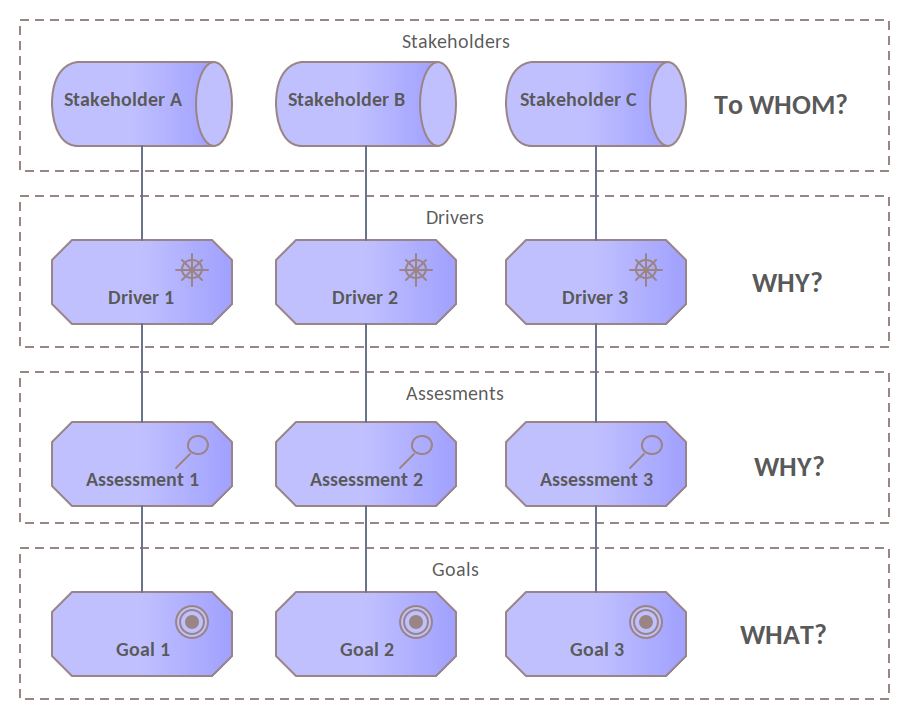
\includegraphics[width=0.7\textwidth]{images/views/Motivation view.png}
		\caption{The layered motivation structure}
		\label{fig:morivation-structure}
	\end{figure}
	
	\textit{Stakeholders} have associated interests, concerns or drivers, which represent internal or external conditions that motivate an organisation to define goals \citep{archimate3.1}.
	
	
	%	\begin{wrapfigure}{r}{0.65\textwidth}
	%		\centering
	%		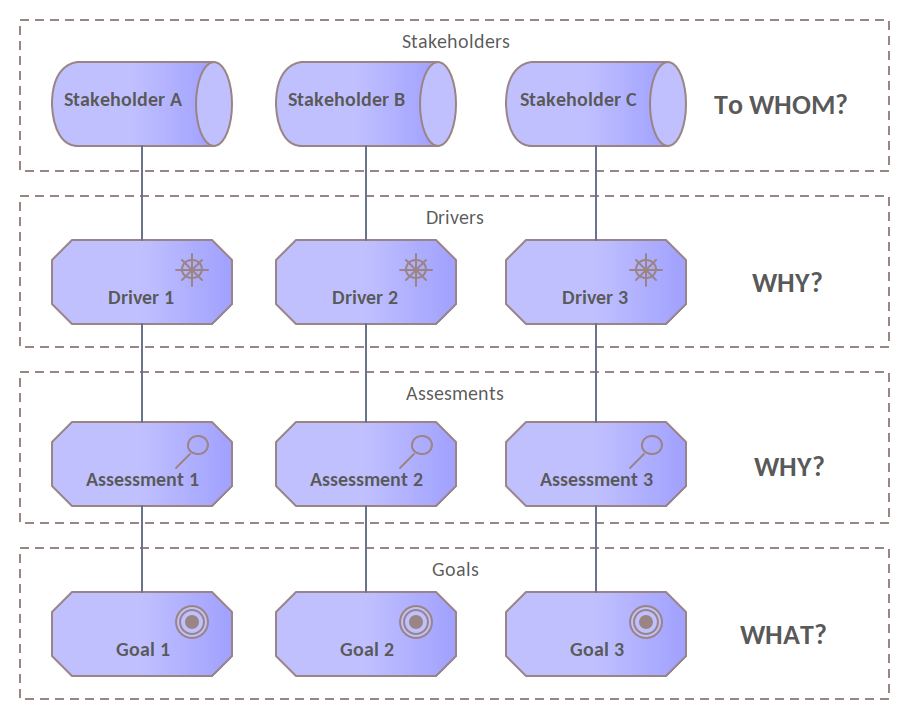
\includegraphics[width=0.67\textwidth]{images/views/Motivation view.png}
	%		\caption{The layered motivation structure}
	%	\end{wrapfigure}
	 
	\textit{Assessments} represent results of analysis of the state of affairs with respect to a driver. They reveal strengths and weaknesses, opportunities or threats to an area of interest \citep{archimate3.1}.
	
	Assessments are associated with goals which represent a high-level statement of intent, plus direction to desired end state for an organisation and its stakeholders \citep{archimate3.1}. 
	
	Next we present the SU motivation structure spread over several sections.
	
	\section{Stakeholders and their roles}
	
	The Standardisation Unit involves multiple stakeholders. We could enumerate them; however, the list would  be long and is outside the scope of this exercise. Instead, we highlight the most important ones and, in addition, we group them based on the role they play in interaction with SU. In Figure \ref{fig:stakehodlers-roles} the roles are depicted as aggregate stakeholders in a grouping frame in the middle of the figure. Above the roles are positioned the most important external stakeholders, while below the stakeholders from the PO are enumerated.
	
	\begin{figure}[!h]
		\centering
		\includegraphics[width=0.8\textwidth]{images/motivation/Stakeholders & Roles.png}
		\caption{The layered motivation structure}
		\label{fig:stakehodlers-roles}
	\end{figure}
	
	The most important external stakeholders are: the European Commission, together with the Secretary General and all of the Commission’s Directorates, the Inter-institutional Metadata and Formats committee (IMFC), Interinstitutional Metadata Maintenance Committee (IMMC), the EuroVoc Committee (Group inter-institutional Lex (GIL)-subgroup EuroVoc), EU Member States (MS) represented by their governments and parliaments, and linguists from different institutions and with a particular interest to the IATE project.
	 
	In Figure \ref{fig:stakehodlers-roles}, the OP stakeholders are placed in organisation-bound context, as the SU is a part of the PO and so its sibling units are not entirely external but are members of the same organisation. The stakeholders within the PO are the various units that use the reference data (e.g. Cellar team, OP Portal team, EurLex team etc.). A Reference Data Steering Committee is scheduled to be formed in the near future in order to coordinate and harmonise the published reference data. And, finally, the Head of the Standardisation Unit (SU) who is in charge of running the enterprise, is also a stakeholder.
	 
	In order to more easily account for the stakeholders' drivers, interests and goals, we grouped them based on their roles in interaction with SU. In Figure \ref{fig:stakehodlers-roles}, the roles are depicted as aggregate stakeholders in a grouping frame in the middle of the figure. The roles include: data consumers, data requester, data disseminators, data overseers and business managers. 
	
	Next we describe each of the roles and briefly enumerate the stakeholders.
	 
	The \textit{data consumers} of published assets are actors who directly engage with and use the published assets in their information systems. Consumers are also considered the actors who use software and services that employs the published assets internally. These consumers are called indirect consumers, while the former ones are called direct consumers.
	
	The \textit{change requester} are agents who require particular content to be available as reference data. 
	
	The \textit{data disseminators} are services and platforms where reference assets are published for broad public consumption.
	
	The \textit{data overseers} are agents who ensure that content satisfying business needs is harmonised, coherent and complete. They are also responsible for the content correctness and harmonisation among multiple stakeholders and its usefulness in the broader context of application. Usually the role of data overseers is performed by the standardisation committees, steering committees and data stewards at large.
	
	\section{Drivers: primary}
	
	We have identified four \textit{primary drivers}, three \textit{secondary drivers} and two \textit{internal efficiency drivers}. The distinction between primary and secondary drivers is based on whether the driver is shared, or not, between the external and internal stakeholders (in this case the business management).
	Figure \ref{fig:primary-drivers} depicts the main stakeholders and their concerns, where the business manager, in this case head of the SU, has the same primary concerns as the main stakeholder roles.
	
	\begin{figure}[h]
		\centering
		\includegraphics[width=0.99\textwidth]{images/motivation/Primary drivers.png}
		\caption{Primary drivers, motivating both, the internal and external stakeholders}
		\label{fig:primary-drivers}
	\end{figure}
	
	For change requesters, the interaction \textit{responsiveness and the speed of the asset life-cycle process} is of primary concern. The sooner the requests are processed and analysed, the sooner they can be implemented, processed and published. The goal of the SU is to rapidly publish overnight change requests, as compared to the current situation when four major publications are scheduled per year allowing also a few urgent ones in between.
	
	The \textit{quality of service} provided by the SU at large, and service consumer satisfaction, is a direct concern for change requesters and data overseers as primary users of various SU services. 
	
	The \textit{quality of data} is of special interest for data overseers as they are directly responsible for this aspect and implicitly of the data consumer satisfaction. The data quality here has a wide meaning covering aspects of formal, semantic and conceptual correctness while also being timely and up-to-date with the business. Besides data overseers, the data users are also interested in high-quality reference data. Data disseminators are indirectly affected by the quality of the data they distribute and also share this interest to a lesser degree. 
	
	The last of the primary drivers is \textit{standardisation, interoperability and adoption}, which is a major concern for data disseminators and data users. This driver covers the adoption of widely-used meta-models, formally well-defined models representing shared conceptualisation of major bodies and organisations, usage and implementation of national and international standards proposed by standardisation bodies (e.g. ISO, W3C, OMG). These standards refer not only to aspects of data representation, but also to protocols, exchange schemes, validation mechanisms and other tools facilitating systemic interoperability. 
	
	\section{Drivers: secondary}
	The secondary drivers are those that are important to both external and internal stakeholders. They are depicted in Figure \ref{fig:secondary drivers}.

	\textit{Steady and uninterrupted IT systems} is a critical driver for the data consumers. Several institutions and OP units have built IT systems which rely on data maintained and published by the SU. Also, this is one dimension of client satisfaction. The SU ensures that data modifications have no impact on external systems, and for that a part of the life-cycle process is dedicated to impact assessment. 
	
	\begin{figure}[h]
		\centering
		\includegraphics[width=1.05\textwidth]{images/motivation/Secondary drivers.png}
		\caption{Secondary drivers, motivating either internal or external stakeholders}
		\label{fig:secondary drivers}
	\end{figure}
	
	\textit{Data reuse} is encouraged at the level of all EU institutions as a means to reduce integration and development costs. The standardisation committees and other responsible parties (the data overseers) are especially interested in this. 
	
	Keeping the knowledge organisation and its structure in a coherent and consistent form is not a trivial task. Reaching a common shared conceptualisation over a given domain is a goal that is difficult to achieve. Nevertheless, it is a precondition if the data is to be reused by multiple parties. Therefore, this constitutes another driver for data overseers. 
	
	Internally, \textit{staff satisfaction} is an important driver for the SU management. Making sure the business and technical teams can fulfil their duties in a flawless and unhindered manner impacts directly their engagement, satisfaction and productivity.
	
	Requests from external clients sometimes do not lead to data changes alone, but result in changes of the technical processes as well, if not developments of additional processes and components. Adapting and configuring the currently-used process is becoming increasingly difficult; therefore, making sure that these operations are possible with minimal effort and that the production process is flexible, represents a driver for SU management. 
	
	Next we have chosen three drivers we considered to be the most important for this exercise, and we present their assessments. 
	
	\section{Assessment: Responsiveness and processing speed}
	
	A number of causes were identified that decrease responsiveness and process speed. 
	
	\begin{figure}[!h]
		\centering
		\includegraphics[width=\textwidth]{images/motivation/Responsiveless & Process Speed.png}
		\caption{The assessment of the responsiveness and processing speed driver}
		\label{fig:responsiveness-and-processing-speed}
	\end{figure}
	
	First of all, execution of the entire publication process (including technical and business processes) is slow. This includes burdening by urgent publication requests, which constitute a technical limitation to processing one asset per day. This assessment was provided by the technical team members. 
	
	To address these problems, we aim to increase the automation level which mostly has an impact on technical aspect of the workflow processes. In addition, the increase of automation level is also to optimise the current workflow process, mostly regarding business aspects, in order to reduce the bottlenecks and streamline production.  
	
	In addition, slow processing of change request cases (internally called tickets) is be due to a limit on the number of cases that can be handled by the business team per week. This process becomes even slower when a change request case involves data modelling and design tasks, which sometimes requires consultation with a technical team member or a knowledge organisation engineer. To reduce this bottleneck, training the team to add knowledge modelling skills or recruiting additional staff with such skills are potential solutions.

	\section{Assessment: Data quality}

    Data quality and, implicitly, consumer satisfaction driver have been assessed with the following issues being identified.
    
	\begin{figure}[!h]
		\centering
		\includegraphics[width=0.9\textwidth]{images/motivation/Data quality.png}
		\caption{The assessment of data quality and data consumer satisfaction}
		\label{fig:data-quality}
	\end{figure}

    The published assets are difficult to adapt by new consumers due to the lack of user manuals. Requests come for both documentation on the conceptual organisation of the asset and the data models used for representing it. We recommend that complete documentation is developed and then published for all assets.
    
    At least for the RDF part of the current publication workflow, the quality assessment is done by technicians undertaking manual checks, ensuring that the transformation processes ran correctly. Therefore, for example, preparing a new version of EuroVoc thesaurus takes days to complete. Moreover, formally-defined validation rules are minimally employed, if at all. The RDF-related processes do not employ SHACL validation, even if the SHACL shape definitions are available. On the XML side, non-semantic validation rules are possible. For these two reasons we propose, as in the previous section, to increase automation and to start employing increasingly more automated validation in order to reduce the time spent by SU team members verifying content before publication. 
    
    Finally, the switch from the XML-based asset sources to RDF-based asset sources is part of the EU trajectory towards public sector linked open data which in turn supports the Public Sector Information (PSI) directive \citep{directive-2019/1024} and the Single Digital Gateway (SDG) initiative \citep{directive-2018/1724}.
    

	\section{Assessment: Service quality}

    A number of complaints have been received, mainly from other OP units, with regards to the quality of services provided by the SU. 

	\begin{figure}[h]
		\centering
		\includegraphics[width=0.8\textwidth]{images/motivation/Service quality.png}
		\caption{The assessment of service quality and service consumer satisfaction}
		\label{fig:service-quality}
	\end{figure}
	
	The complaints are mainly due to the lack of OP internal synchronisation between units, both regarding communication and operational coordination. This is in part linked to a lack of precise knowledge of who the users are and in which manner they engage with assets published by the SU. 
	
	
	To address these two issues, our main recommendation (aligned with SU management vision) is to introduce a control tower-like faculty into the SU, which would take care of synchronisation (communication-wise and operational) with all OP units, and if possible with parties from other institutions and Member States.
	
	Another request often received by the SU is to provide modelling and knowledge organisation services to third party clients: the SU does not currently offer such service. In order to establish the grounds for setting up such service provision in the future, we recommend increasing the number of team members mastering the knowledge modelling and information design domains. 
	
	This brings us to the end of the motivation structure section. While we did not provide an extensive account, we did however identify some SU motivations, drivers and goals that are relevant, directly or indirectly, to the aims of this enterprise architecture.